\documentclass[a4paper]{article}
\usepackage[T2A]{fontenc}
\usepackage[utf8]{inputenc}
\usepackage[russian]{babel}
\usepackage{graphicx}
\usepackage{amsfonts}
\usepackage{amsmath}
\usepackage{wrapfig}
\usepackage{epstopdf}
\usepackage{multirow}
\usepackage{subcaption}
\usepackage{floatrow}
\usepackage[left=2cm,right=2cm,
    top=2cm,bottom=2cm,bindingoffset=0cm]{geometry}

\author{Петров Артём Антонович, группа 721}
\title{Лабораторная работа № 3.4.5 "Петля гистерезиса (динамический метод)"}
\date{04 декабря 2018}

\begin{document}

\maketitle

\textbf{Цель работы:} Изучение вольт-амперной характеристики тлеющего разряда; изучение свойств плазмы методом зондовых характеристик.

\textbf{В работе ипользуются:} стеклянная газоразрядная трубка, наполненная изотопом неона, высоковольтный источник питания(ВИП), источник питания постоянного тока, делитель напряжения, резистор, потенциометр, амперметры, вольтметры, переключатели.
 
\textbf{Основные формулы:}
\begin{equation}
	kT_e = \frac{1}{2} \frac{e I_{i\mbox{н}}}{\frac{dI}{dU}|_{U=0}}
\end{equation}
\begin{equation}
	I_{i\mbox{н}} =  0,4 n e S \sqrt{\frac{2kT_e}{m_i}}
\end{equation}
\begin{equation}
	\omega_p = \sqrt{\frac{n_e e^2}{\varepsilon_0 m_e}}
\end{equation}
\begin{equation}
	r_d = \sqrt{\frac{k T_i \varepsilon_0}{n e^2}}
\end{equation}
\begin{equation}
	N_d = n_i \frac{4}{3} \pi r_d^3
\end{equation}
\begin{equation}
	P = nkT
\end{equation}
\textbf{Ход работы:}\\
Снимая вольтамперную характеристику разряда, получаем($\sigma_U = 0,01$В, $\sigma_{I_p} = 0,2$мА):
  % используем стиль, в котором подписи таблиц 
  % сверху и выравнены "по верху"
  \floatsetup[table]{style=Plaintop,floatrowsep=qquad}
  %
  % Теперь сами таблицы в ряд
  \begin{table}[!h]
  \begin{floatrow}
   % первая таблица
   \ttabbox[\FBwidth]{}%
           {
\begin{tabular}{|c|c|}
\hline
$U_1$, В & $I_p$,мА \\ \hline
33,76   & 0,6     \\ \hline
33,06   & 0,8     \\ \hline
32,51   & 1,0       \\ \hline
32,13   & 1,2     \\ \hline
31,82   & 1,4     \\ \hline
31,01   & 1,6     \\ \hline
30,09   & 1,8     \\ \hline
29,66   & 2,0       \\ \hline
29,10    & 2,2     \\ \hline
28,61   & 2,4     \\ \hline
28,25   & 2,6     \\ \hline
27,96   & 2,8     \\ \hline
\end{tabular}
    }
   % вторая таблица
   \ttabbox[\FBwidth]{}%
           {
\begin{tabular}{|c|c|}
\hline
$U_1$, В & $I_p$,мА \\ \hline
27,78   & 3,0       \\ \hline
27,60    & 3,2     \\ \hline
27,42   & 3,4     \\ \hline
27,35   & 3,6     \\ \hline
27,22   & 3,8     \\ \hline
27,18   & 4,0       \\ \hline
27,22   & 4,2     \\ \hline
27,25   & 4,4     \\ \hline
27,25   & 4,6     \\ \hline
27,22   & 4,8     \\ \hline
27,18   & 5,0       \\ \hline
\end{tabular}
           }
\end{floatrow}
\end{table}

\newpage
\begin{figure}[!h]
\centering
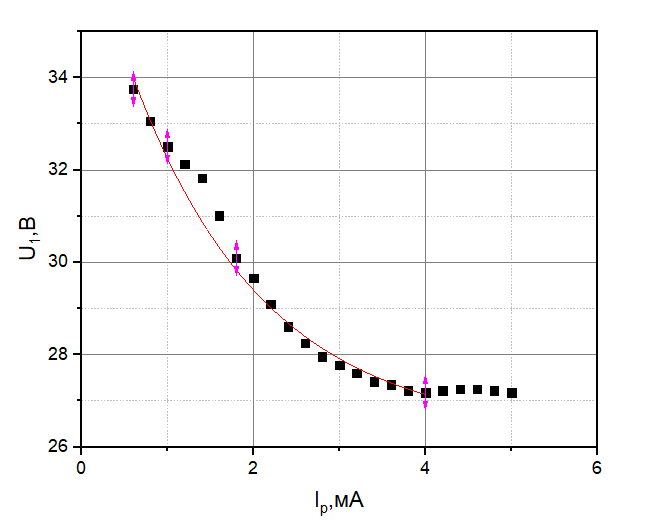
\includegraphics[width = 0.55\textwidth]{graph_1.png}
\end{figure}

Откуда находим, что $R_{max} = -3500$ Ом. 

Далее проведем измерения зондовых характеристик при разных токах(во всех измерениях $\sigma_U = 0,01$В ,а $\sigma_I = 0,1$ мкА):

  % используем стиль, в котором подписи таблиц 
  % сверху и выравнены "по верху"
  \floatsetup[table]{style=Plaintop,floatrowsep=qquad}
  %
  % Теперь сами таблицы в ряд
  \begin{table}[!h]
  \begin{floatrow}
   % первая таблица
   \ttabbox[\FBwidth]{}%
           {
\begin{tabular}{|c|c|}
\hline
$U_2$, В &$ I_2$, мкА \\ \hline
25,08   & 118,7     \\ \hline
22,04   & 115,7     \\ \hline
19,01   & 112,5     \\ \hline
15,97   & 108,8     \\ \hline
12,99   & 103,5     \\ \hline
10,02   & 94,8      \\ \hline
8,00       & 86,1      \\ \hline
6,00      & 74,2      \\ \hline
4,06    & 59,1      \\ \hline
2,08    & 34,3      \\ \hline
0,17    & 16,3      \\ \hline
-0,23   & -9,4      \\ \hline
-2,00      & -12,3     \\ \hline
-4,02   & -34,3     \\ \hline
-6,00      & -51,8     \\ \hline
-8 ,00     & -65,1     \\ \hline
-10,00     & -74,8     \\ \hline
-13,03  & -84,2     \\ \hline
-16,07  & -89,7     \\ \hline
-19,08  & -93,3     \\ \hline
-22,02  & -96,6     \\ \hline
-25,08  & -99,6     \\ \hline
\end{tabular}
\caption{$I_p = 5$мА}
    }
   % вторая таблица
   \ttabbox[\FBwidth]{}%
           {
\begin{tabular}{|c|c|}
\hline
$U_2$, В &$ I_2$, мкА \\ \hline
-25,08  & -72,4     \\ \hline
-22,05  & -70,1     \\ \hline
-19,04  & -67,9     \\ \hline
-16,11  & -65,9     \\ \hline
-13,09  & -62,0       \\ \hline
-10,07  & -55,6     \\ \hline
-7,99   & -48,2     \\ \hline
-5,98   & -37,9     \\ \hline
-3,96   & -24,0       \\ \hline
-1,97   & -7,2      \\ \hline
-1,03   & -1,5      \\ \hline
0,74    & 19,5      \\ \hline
1,98    & 30,8      \\ \hline
4,01    & 46,7      \\ \hline
5,95    & 58,7      \\ \hline
8,00       & 68,0        \\ \hline
10,00      & 74,3      \\ \hline
12,95   & 80,4      \\ \hline
16,02   & 84,3      \\ \hline
18,96   & 87,1      \\ \hline
22,02   & 89,8      \\ \hline
25,08   & 92,5      \\ \hline
\end{tabular}
\caption{$I_p = 4$мА}
           }
   %третья таблица
   \ttabbox[\FBwidth]{}%
           {
\begin{tabular}{|c|c|}
\hline
$U_2$, В &$ I_2$, мкА \\ \hline
-25,08  & -51,3     \\ \hline
-21,98  & -49,5     \\ \hline
-19,08  & -48,1       \\ \hline
-16,01  & -46,3     \\ \hline
-12,96  & -43,9     \\ \hline
-10,00     & -39,7     \\ \hline
-8,01   & -34,6     \\ \hline
-6,01   & -27,1     \\ \hline
-4,00      & -16,8     \\ \hline
-2,05   & -4,5      \\ \hline
-0,85   & -4,1        \\ \hline
0,84    & 16,4      \\ \hline
2,00       & 24,2      \\ \hline
3,98    & 35,8      \\ \hline
6,05    & 45,1      \\ \hline
8,03    & 51,5      \\ \hline
10,08   & 55,9      \\ \hline
12,97   & 59,6      \\ \hline
15,97   & 62,2      \\ \hline
18,98   & 64,3      \\ \hline
21,98   & 66,4      \\ \hline
25,08   & 68,6      \\ \hline
\end{tabular}
\caption{$I_p = 3$мА}
    }
 %четвертая таблица
   \ttabbox[\FBwidth]{}%
           {
\begin{tabular}{|c|c|}
\hline
$U_2$, В &$ I_2$, мкА \\ \hline
25,08   & 36,1        \\ \hline
21,98   & 34,7      \\ \hline
19,10    & 33,5      \\ \hline
16,01   & 32,2      \\ \hline
12,93   & 30,8      \\ \hline
10,03   & 28,9      \\ \hline
8,07    & 26,8      \\ \hline
6,03    & 23,6      \\ \hline
4,00      & 19,1        \\ \hline
2,01    & 13,1      \\ \hline
0,48    & 9,6       \\ \hline
-0,94   & -2,6      \\ \hline
-2,07   & -1,3      \\ \hline
-4,06   & -7,7      \\ \hline
-6,00      & -12,7     \\ \hline
-8,02   & -16,5     \\ \hline
-9,93   & -18,8     \\ \hline
-12,98  & -20,7     \\ \hline
-15,98  & -21,6     \\ \hline
-19,03  & -22,3     \\ \hline
-22,00     & -23,1       \\ \hline
-25,08  & -23,7     \\ \hline
\end{tabular}
\caption{$I_p = 1,48$мА}
           }
\end{floatrow}
\end{table}

\newpage

\begin{figure}[!h]
\centering
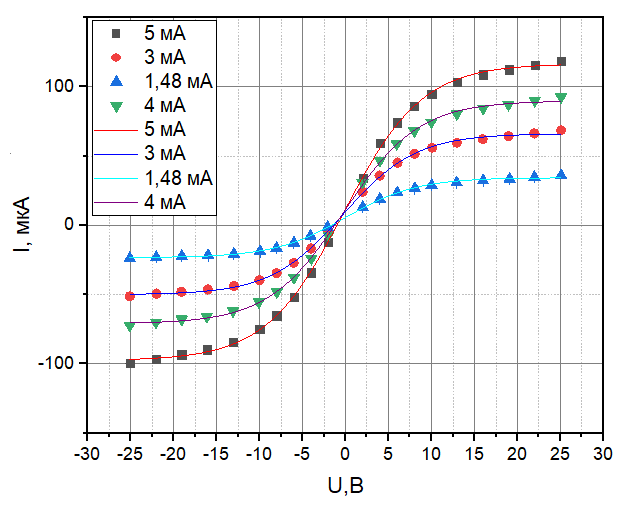
\includegraphics[width = 0.57\textwidth]{graph_2.png}
\end{figure}

\begin{figure}[!h]
\centering
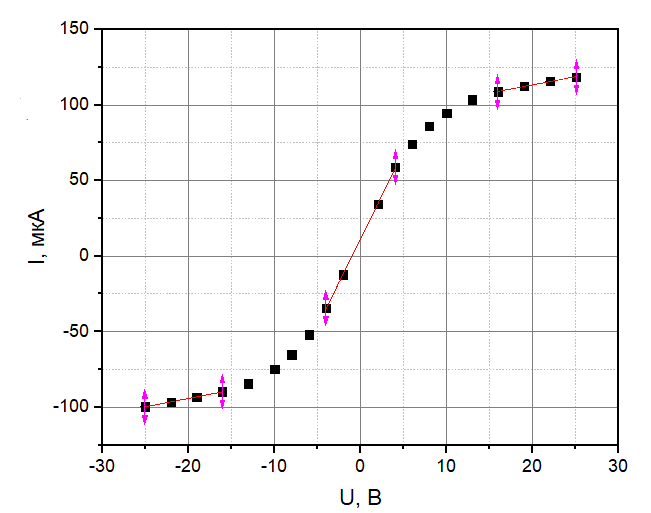
\includegraphics[width = 0.57\textwidth]{graph_3.png}
\end{figure}

\begin{figure}[!h]
\centering
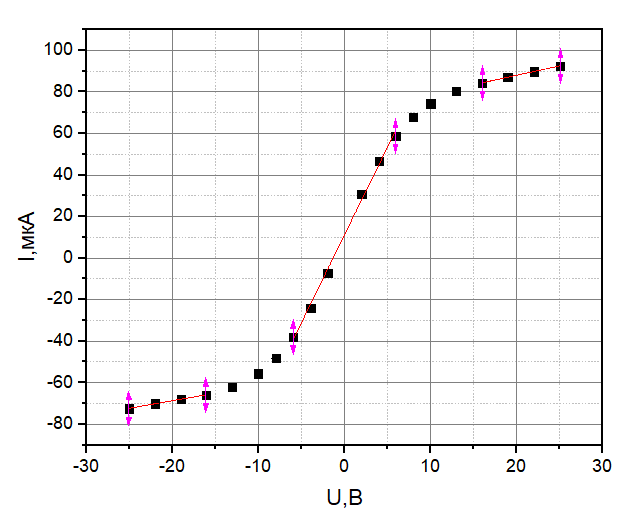
\includegraphics[width = 0.57\textwidth]{graph_4.png}
\end{figure}


\begin{figure}[!h]
\centering
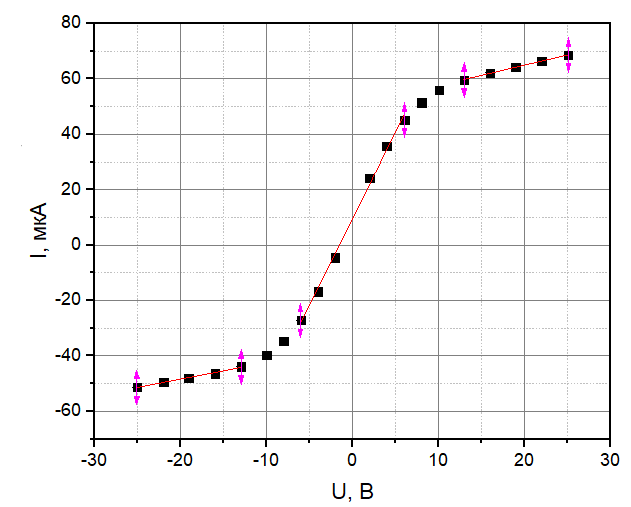
\includegraphics[width = 0.59\textwidth]{graph_5.png}
\end{figure}


\begin{figure}[!h]
\centering
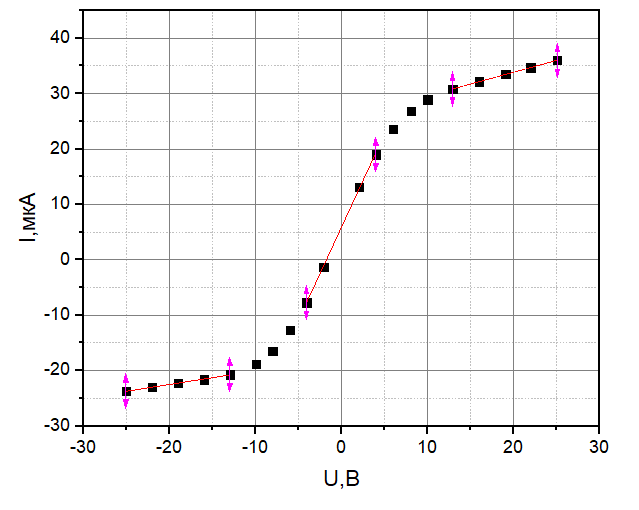
\includegraphics[width = 0.59\textwidth]{graph_6.png}
\end{figure}

\begin{figure}[!h]
\centering
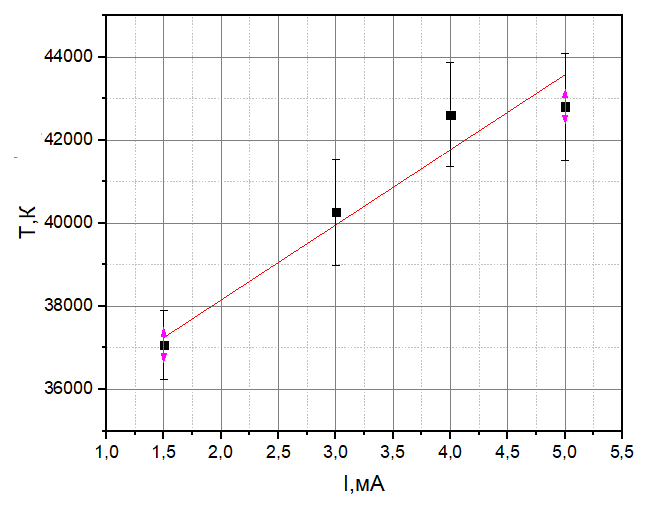
\includegraphics[width = 0.59\textwidth]{graph_7.png}
\end{figure}

\begin{figure}[!h]
\centering
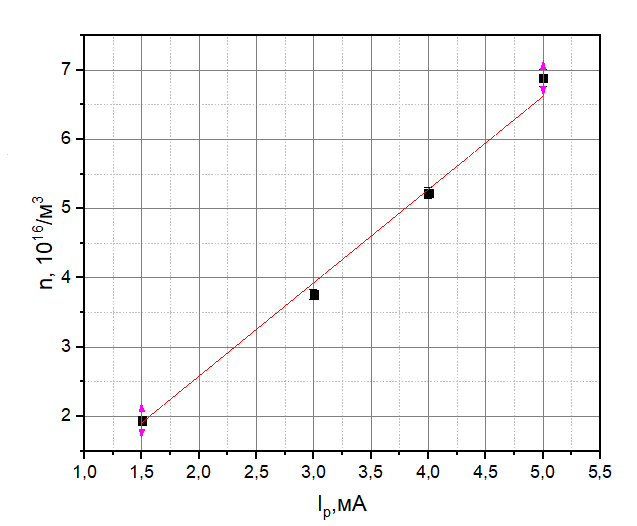
\includegraphics[width = 0.55\textwidth]{graph_8.png}
\end{figure}

\begin{table}[!h]
\begin{tabular}{|c|c|c|c|c|c|c|c|}
\hline
$R_{max}$, Ом             & $I_p$,мА & $kT_e$, эВ & $n_e, 10^{10}/\mbox{см}^3$ & $\omega, 10^{10} \mbox{рад}/\mbox{с}$ & $r_d, \mbox{см}*10^{-4}$ & $N_d$   & $\alpha*10^6$ \\ \hline
\multirow{4}{*}{-3500} & 5,00 & $3,69 \pm 0,11$   & $6,89 \pm 0,12$                                            & $1,479 \pm 0,013$                           & $4,558 \pm 0,040$        & $27,3 \pm 0,9$ & $2,851 \pm 0,050$                       \\ \cline{2-8} 
                       & 4,00 & $3,68 \pm 0,11$   & $5,23 \pm 0,08$                                            & $1,288 \pm 0,010$                          & $5,233 \pm 0,040$        & $31,4 \pm 0,9$ & $2,164 \pm 0,034$                      \\ \cline{2-8} 
                       & 3,00 & $3,47 \pm 0,11$  & $3,76 \pm 0,07$                                            & $1,093 \pm 0,010$                          & $6,170 \pm 0,058$         & $37,0 \pm 1,3$ & $1,556 \pm 0,029$                       \\ \cline{2-8} 
                       & 1,48 & $3,20 \pm 0,07$   & $1,94 \pm 0,03$                                            & $0,785 \pm 0,005$                           & $8,590 \pm 0,063$         & $51,5 \pm 1,4$ & $0,803 \pm 0,012$                       \\ \hline
\end{tabular}
\caption{$\sigma_{I_p} = 0,02$ мА}
\end{table}


\textbf{Вывод:}Таким образом, зондовый метод исследования плазмы является удобным. С помощью зондовых характеристик мы смогли узнать некоторые параметры плазмы.

\end{document}